
 
 
		
		
		

	\subsection{Jacobi Matrix \small{ (erklärt durch Beispiel)}}
		
		
        Die Jacobi-Matrix eines Roboterarms beschreibt die Abbildung von
        Gelenkgeschwindigkeiten auf die Lineargeschwindigkeit des TCP
        und die zeitlichen Änderungen der Orientierung des End-Effektors
        bezogen auf ein Referenzkoordinatensystemk z.B. auf das
        Basiskoordinatensystem O auf. \\
        In der Positionsbeschreibung werden alle Parameter die einen Einfluss 
       auf den Greifer haben aufgestellt und dann für die Jakobi-Matrix nach diesen Partiell abgeleitet. \\
    
	     \begin{minipage}{5cm}
	        Für die Jacobi Matrizen \\
	        empfehlen sich \\
	        Kurzschreibweisen
	        \end{minipage}
			\begin{minipage} {8cm}
            
	        $ c_{12}=cos(\theta_{1} + \theta_{2}) $ \\
	        $ s_{12}=sin(\theta_{1} + \theta_{2}) $
	        
	        \end{minipage}\\ \\
	     \begin{minipage}{12cm}
	     \subsubsection{Vorwärtskinematik}
	     	Geg: Gelenkkoordinaten und Geschwindigkeiten: $q ; \dot{x}$ \\
			Ges: Geschwindigkeit des Endeffektors: $\dot{X} = [\dot{x} \dot{y} \dot{z}
			\dot{\alpha} \dot{\beta} \dot{\gamma}]^{T}$ \\ 
			Lsg: Jacobi-Matrix $ \Longrightarrow \dot{X}=J(q)*\dot{q}$ \\ \\
			Positionsbeschreibung des Endeffektors: \\
	     $
	    			\begin{bmatrix} 
				    	x_{e} \\
				        y_{e} \\                             
				    \end{bmatrix}
					=
					\begin{bmatrix} 
				    	d_{2}cos\theta_{1}+l_{3}cos(\theta_{1}+\theta_{3}) \\
				        d_{2}sin\theta_{1}+l_{3}sin(\theta_{1}+\theta_{3}) \\                              
				    \end{bmatrix} $ und $ \Phi_{e}=\theta_{1}+\theta_{3} \\ \\$
			Jacobi-Matrix: \\ $
				J = 
					\begin{bmatrix} 
				    	\frac{\partial{x_{e}}}{\partial{\theta_{1}}} & 
				    	\frac{\partial{x_{e}}}{\partial{d_{2}}} & 
				    	\frac{\partial{x_{e}}}{\partial{\theta_{3}}} \\
				    	\frac{\partial{y_{e}}}{\partial{\theta_{1}}} & 
				    	\frac{\partial{y_{e}}}{\partial{d_{2}}} & 
				    	\frac{\partial{y_{e}}}{\partial{\theta_{3}}} \\
				    	\frac{\partial{\Phi_{e}}}{\partial{\theta_{1}}} & 
				    	\frac{\partial{\Phi_{e}}}{\partial{d_{2}}} & 
				    	\frac{\partial{\Phi_{e}}}{\partial{\theta_{3}}} \\ 
				    \end{bmatrix} \\
			$ \space  $	=
					\begin{bmatrix} 
					    	-d_{2}sin(\theta_{1})-l_{3}sin(\theta_{1}+\theta_{3}) & 
					    	cos(\theta_{1}) & 
					    	-l_{3}sin(\theta_{1}+\theta_{3}) \\
					        d_{2}cos(\theta_{1})+l_{3}cos(\theta_{1}+\theta_{3}) & 
					        sin(\theta_{1}) & 
					        l_{3}cos(\theta_{1}+\theta_{3}) \\
					        1 & 
					        0 & 
					        1 \\                            
					    \end{bmatrix}$		
			\end{minipage}
			\begin{minipage}{8cm}
			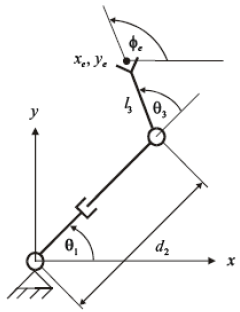
\includegraphics[width=5cm]{./bilder/jacobi-bsp.png}
			\end{minipage}
			
			\subsubsection{Rückwertskinematik}
			Geg: Geschwindigkeiten des Endeffektors: $\dot{x}$ \\
			Ges: Gelenkgeschwindigkeiten: $\dot{q}$ \\
			Lsg: Jacobi-Matrix $ \Longrightarrow \dot{q}=J^{-1}\dot{x}$ \\ \\
			Singularität: \\
			Die Jacobi-Matrix kann in singulären Stellungen
			nicht invertiert werden (d.h. die Determinante von J ist 0) und der Roboter
			kann in bestimmten Richtungen keine Bewegungen
			vornehmen. \\
			Mehr: Skript-Kinematik (S.11 ff) \& UB5 Bahnplanung (Aufg. 2))
			
\subsection{Denavit-Hartenberg}
\begin{minipage}{19cm}
	\textbf{Ablauf:}
	\begin{enumerate}{\setlength{\itemsep}{0cm}\setlength{\parsep}{0cm} \setlength{\topsep}{0cm}}
      \item Gelenke nummerieren in aufsteigender Reihenfolge. Starten in der Basis mit Nummer null.
      \item Jeden Achskörper mit Koordinatensystem belegen.
      \item Die $z_i$-Koordinatenachse muss mit der i+1 Gelenkachse zusammenfallen.
      \item Die $x_i$-Achse liegt entlang der Normalen zwischen der $z_{i-1}$ und $z_i$-Achse und zeigt vom Gelenk i zum Gelenk i+1.
      \item $y_i$-Achsen vervollständigen mit der Rechten-Hand-Regel. (x:Daumen, y:Zeigfinger, z:Mittelfinger)
      \item Festlegen der DH-Parameter (siehe DH-Parameter) und eintragen in DH-Tabelle.
      \item DH-Matrizen berechnen und miteinander mulitplizieren.
    \end{enumerate}
    \vspace{0.2cm}
\end{minipage}\\

\begin{minipage}{19cm}
	\textbf{Anmerkung Koordinatensysteme:}
	\begin{itemize}\itemsep0pt
      \item $z_i$-Achse muss grundsätzlich mit Bewegungsachse des zugehörigen Achskörper zusammenfallen.
      		Bei Rotationsgelenken gilt die Rechte-Handregel für Drehungen. 
      \item Ursprung des Koordinatensystems im Schnittpunkt der Bewegungsachsen.
    \end{itemize}
    \vspace{0.2cm}
\end{minipage}\\

\begin{minipage}{19cm}
	\textbf{DH-Parameter:}\\ \\
	\begin{tabular}{l l}
  		Linklänge $a_i$ (Fixwert): 				& Für $z_{i-1}$- und $z_i$-Achse wird die gem. Normale mit Länge $a_i$ in $x_i$-Richtung gemessen.\\
  		Linkdrehung $\alpha_{i}$ (Fixwert):		& Drehwinkel um $x_i$-Achse bis $z_{i-1}$- und $z_i$-Achse in gleiche Richtung zeigen.\\
  		Link Offset $d_i$ (Variable):			& Abstand von $x_{i-1}$- und $x_i$-Achse entlang der $z_{i-1}$-Achse.\\
 	 	Gelenkwinkel $\theta_{i}$ (Variable):	& Drehwinkel um $z_{i-1}$-Achse bis $x_{i-1}$- und $x_i$-Achse in gleiche Richtung zeigen.\\
    \end{tabular}
	\vspace{0.5cm}
\end{minipage}\\
\begin{minipage}{19cm}
\textbf{DH-Tabelle:}\\ \\
	\begin{minipage}{10cm}
    	\renewcommand{\arraystretch}{1.1}
			\begin{tabular}{| c | c | c | c | c |}
				\hline
					\textbf{Gelenk Nr.}
					& \textbf{Linklänge $a_i$}
					& \textbf{Linkdrehung $\alpha_{i}$}
					& \textbf{Link Offset $d_i$} 
					& \textbf{Gelenkwinkel $\theta_{i}$}\\
				\hline
					i
					&&&& \\
				\hline
					i+1
					&&&& \\
				\hline
					\ldots
					&&&&\\
				\hline
			\end{tabular}
		\renewcommand{\arraystretch}{1}
		\vspace{0.5cm}
    \end{minipage}
\end{minipage}\\
\begin{minipage}{19cm}
	\textbf{DH-Matrizen:}\\ \\
	$ ^{i-1}_{i}T =
	\begin{bmatrix}
    	cos(\theta_i) & -sin(\theta_i) cos(\alpha_i) &  sin(\theta_i) sin(\alpha_i) & a_i cos(\theta_i)\\
    	sin(\theta_i) &  cos(\theta_i) cos(\alpha_i) & -cos(\theta_i) sin(\alpha_i) & a_i sin(\theta_i)\\
    	0			  &  sin(\alpha_i)				 &  cos(\alpha_i)				& d_i\\
    	0			  &  0							 &  0							& 1\\
    \end{bmatrix}
\qquad
	 ^{0}_{n}T = \prod\limits_{i=1}^{n} \quad ^{i-1}_{i}T(\theta_{i}) = ^{0}_{1}T \cdot ^{1}_{2}T \cdot \ldots \cdot ^{n-1}_{n}T $
\end{minipage}\\\\

\begin{minipage}{3cm}
\textbf{Beispiel:}
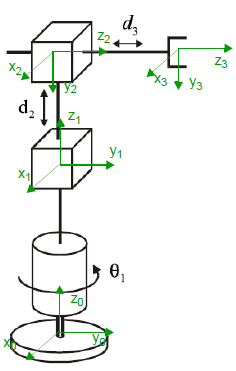
\includegraphics[width=4cm]{./bilder/denavit_grafik.png} \\
\end{minipage}
\begin{minipage}{6cm}
$\alpha_{i} \Longrightarrow $ Linkdrehung  \\
$ a_{i} \Longrightarrow $ Linklänge [Achsenabstand] \\
$ d_{i} \Longrightarrow $ Offset \\
$ \Theta_{i} \Longrightarrow $ Gelenkwinkel \\ 
\end{minipage}
\begin{minipage}{8cm}
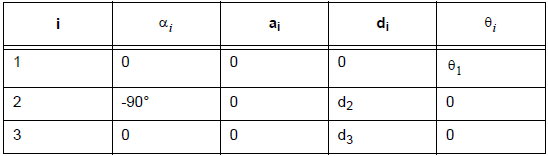
\includegraphics[width=9cm]{./bilder/denavit_tabelle.png} \\
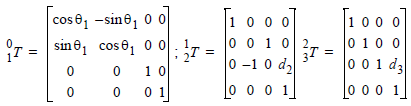
\includegraphics[width=9cm]{./bilder/denavit_matrix.png} \\
\end{minipage} \\
